$subject$=Дополнительные главы \\ высшей математики
$date$=04.04.2025
$teacher$=Лекции Далевской О. П.

Свойства комплексного интеграла:

\begin{enumerate}[label*=\arabic*$^\circ$ ]
    \item Линейность
    \item Аддитивность
    \item Смена знака: $\int_{K^+} = - \int_{K^-}$
    \item Оценка, модуль: $\left|\int_K\right| \leq \int_K |f(z)| dz$
    \item $\int_K f(z) dz \overset{z = g(w)}{=} \int_C f(g(w)) g^\prime (w) dw = \left[\text{В частности переход к параметру } t\right] = 
    \int_{C(t)} f(t) g^\prime(t) dt$
\end{enumerate}

\Ex $I = \int_{K : |z - z_0| = \rho} \frac{dz}{z - z_0} \overset{z - z_0 = \rho e^{i\varphi}}{=} \int_K \frac{d\rho e^{i\varphi}}{\rho e^i\varphi} = 
\int_K \frac{i e^{i\varphi} d\varphi}{e^i\varphi} = i \int_0^{2\pi} d\varphi = 2\pi i$

Интеграл $I$ не зависит от радиуса и центра окружности (то есть контура интегрирования), то есть
интеграл функции $\frac{1}{z - z_0}$ будет равен $2\pi i$ для любой окружности в качестве контура 

\subsubsection{6.2. Теорема Коши}

\begin{MyTheorem}
    \ThNs{1} $f(z)$ аналитическая и однозначная в односвязной области $D$

    Если $f(z)$ непрерывна на $\Gamma_D$, то $\oint_{\Gamma_D} f(z) dz = 0$
\end{MyTheorem}

\begin{MyProof}
    \begin{center}
        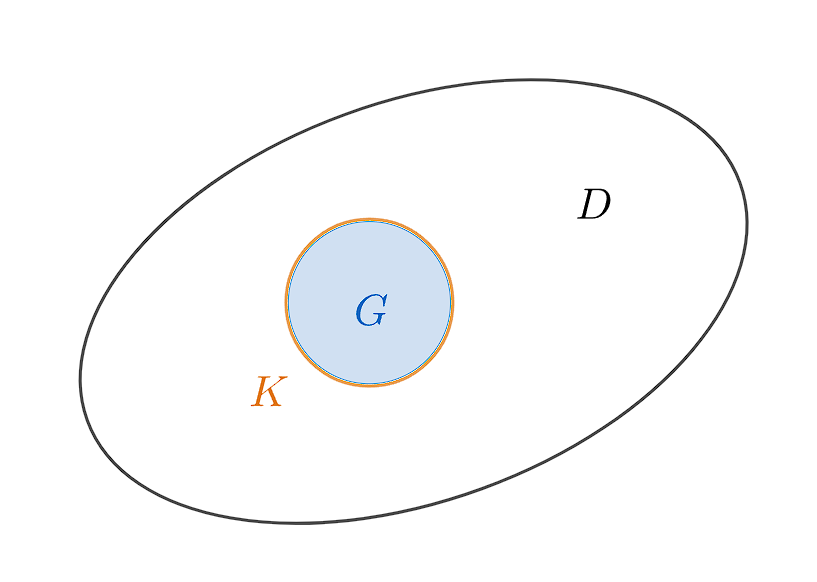
\includegraphics[width=8cm]{addchapters2/images/addchapters2_2025_04_04_1}
    \end{center}

    Запишем интеграл по контуру $K \subset D$ ($K$ - кусочно гладкая):

    $\int_K f(z) dz = \int_K u dx - vdy + i \int_K u dy + v dx = I_1 + I_2 i$

    $I_1 = \int_K \underbrace{P(x, y)}{\underbrace{u(x, y)}} dx - \underbrace{Q(x, y)}{\underbrace{v(x, y)}} dy = 
    \begin{bmatrix}f(z)\text{ - аналитическая} \Longrightarrow \\ u_x, u_y, v_x, v_y \text{ существуют} \\ \text{и непрерывны}\end{bmatrix} = 
    \underset{\text{Формула Грина}}{\iint_G \left(\frac{\partial Q}{\partial x} - \frac{\partial P}{\partial y}\right) dxdy} = 
    \iint_G \left(-\frac{\partial v}{\partial x} - \frac{\partial u}{\partial y}\right) dxdy = 
    \iint_G \left(\frac{\partial u}{\partial y} - \frac{\partial u}{\partial y}\right) dxdy = 0$

    Аналогично $I_2 = \int_k udy + vdx = \iint_G \left(\frac{\partial u}{\partial x} - \frac{\partial v}{\partial y}\right) dxdy = 
    \iint_G \left(\frac{\partial u}{\partial x} - \frac{\partial u}{\partial x}\right) dxdy = 0$

    Таким образом, $\oint_{K \subset D} f(z) dz = 0$ - формула Коши

    Так как $f(z)$ непрерывна на $\Gamma_D$, то можно взять $K = \Gamma_D$
\end{MyProof}

\Nota Получим, что интеграл по любому замкнутому $\Gamma_D$ контуру в области аналитичности равен нулю

То есть $\int_{AB} f(z) dz$ в условиях \ThNs{1} не зависит от пути, и его можно решать как $\int_{AB} = \int_A^B$

\Nota Обобщим \ThNs{1} на многосвязную область. Выколотые области тоже имеют границы, которые включены в границу всей области

\begin{MyTheorem}
    % https://www.geogebra.org/calculator/ujuysjcp
    
    \begin{center}
        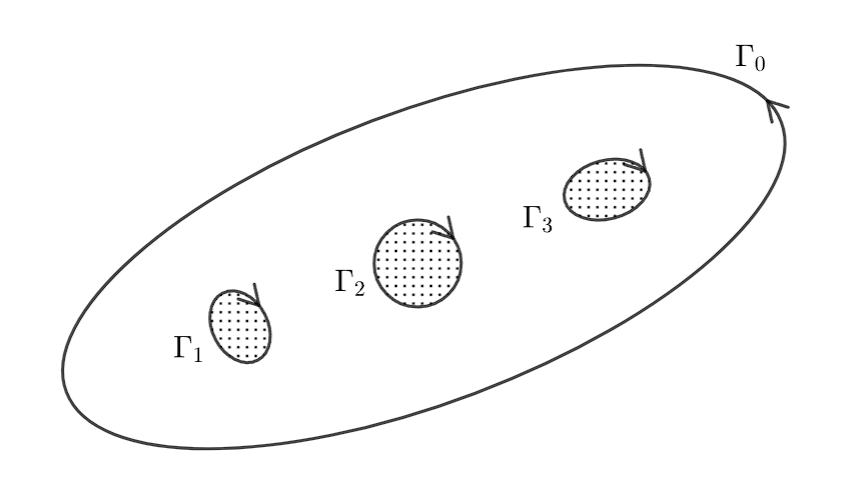
\includegraphics[width=10cm]{addchapters2/images/addchapters2_2025_04_04_2}
    \end{center}
    
    \ThNs{2} Дана многосвязная область $D$, $f(z)$ - аналитична в $D$ и непрерывна на $\Gamma_D$


    Граница $\Gamma_D = \Gamma_0 \cup \Gamma_1 \cup \Gamma_2 \cup \dots \cup \Gamma_n$, где положительным обходом области
    считается тот, при котором область обхода слева

    Тогда $\int_{\Gamma_D^+} f(z) dz = 0$ или $\int_{\Gamma_0 \CounterClockwiseArrow} f(z) dz = \sum_{i = 1}^n \int_{\Gamma_i \CounterClockwiseArrow} f(z) dz$ 
\end{MyTheorem}


\begin{MyProof}
    Сделаем разрезы как на картинке. 
    Разрезы превратили область $D$ в односвязную с границей $\Gamma^\prime = \Gamma_0 \cup (\gamma_1^+ \cup \gamma_1^- \cup \Gamma_1) \cup \dots = \Gamma_0 \cup \bigcup_{i = 1}^n (\gamma_i^+ \cup \gamma_i^- \cup \Gamma_i)$

    \begin{center}
        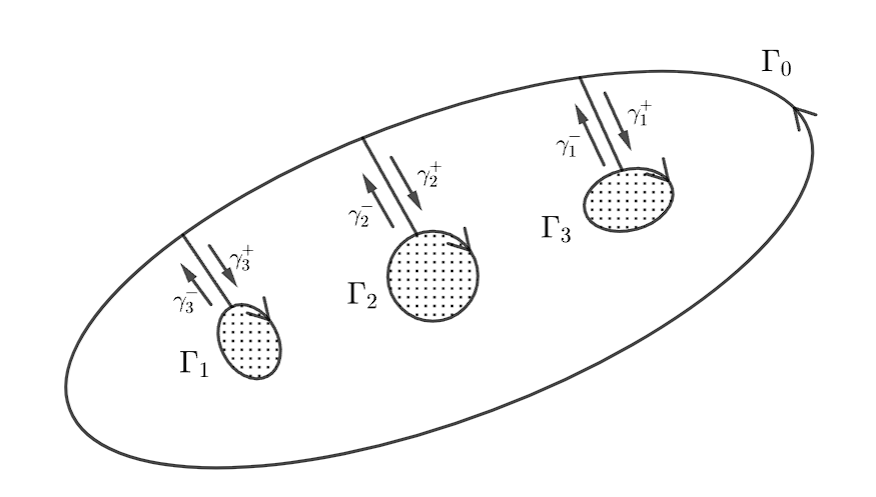
\includegraphics[width=10cm]{addchapters2/images/addchapters2_2025_04_04_3}
    \end{center}

    По \ThNs{1} $\int_{\Gamma^\prime} f(z) dz = 0 \Longleftrightarrow \int_{\Gamma_D} f(z) dz + \int_{\gamma^+_1} f(z) dz + \int_{\gamma^-_1} f(z) dz + \int_{\Gamma_1} f(z) dz + \dots = 0$

    Но $\int_{\gamma_1^+} = - \int_{\gamma_1^-}$, поэтому $\int_{\Gamma_D^+} = \sum \int_{\Gamma_i^-}$ или $\int_{\Gamma_0 \CounterClockwiseArrow} = \sum \int_{\Gamma_i \CounterClockwiseArrow}$
\end{MyProof}

% https://www.geogebra.org/calculator/rdsykgz5

\begin{wrapfigure}{R}{0pt}
    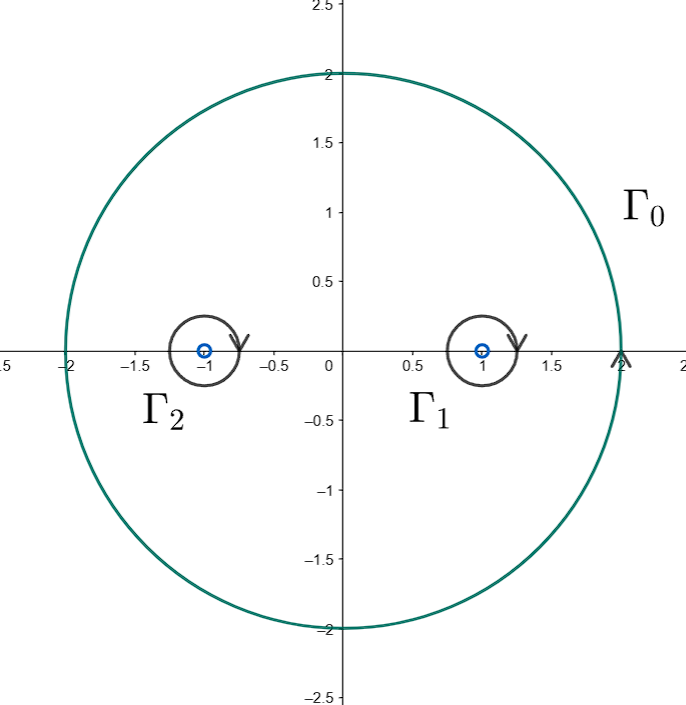
\includegraphics[width=4.5cm]{addchapters2/images/addchapters2_2025_04_04_4}
\end{wrapfigure}

\Ex $\int_{|z| = 2} f(z) dz$

По \ThNs{2} $\int_{\Gamma_0 \CounterClockwiseArrow} f(z) dz + \int_{\Gamma_1 \ClockwiseArrow} f(z) dz + \int_{\Gamma_2 \ClockwiseArrow} f(z) dz = 0$

Тогда $\int_{|z| = 2 \CounterClockwiseArrow} f(z) dz = \int_{|z - 1| = \rho_1 \CounterClockwiseArrow} f(z) dz + \int_{|z + 1| = \rho_2 \CounterClockwiseArrow} f(z) dz$,
где $\rho_1$, $\rho_2$ - радиусы бесконечно малой длины 

\subsubsection{6.3. Неопределенный интеграл}

\Mem По теореме Барроу $\Phi(x) = \int_{x_0}^x f(t) dt$ - интеграл с переменным верхним пределом

Тогда $\Phi(x)$ - дифференцируема, и $\Phi^\prime(x) = f(x)$, то есть $\Phi(x)$ - первообразная $f(x)$

\begin{MyTheorem}
    \Ths $f(z)$ непрерывна в односвязной области $D$ и $\forall \Gamma \subset D \ \int_\Gamma f(z) dz = 0$

    Тогда при фиксированном $z_0 \in D \ \Phi(z) = \int_{z_0}^z f(\zeta) d\zeta$ аналитична в $D$ и $\Phi^\prime(z) = f(z)$
\end{MyTheorem}

\begin{MyProof}
    Если $\forall \Gamma \ \int_\Gamma f(z) dz = 0$, то $\Phi(z) = \int_{z_0}^z F(\zeta) d\zeta$ - интеграл, не зависящий от пути, а только от $z_0$ и $z$

    Рассмотрим $\frac{\Phi(z + \Delta z) - \Phi(z)}{\Delta z} = \frac{1}{\Delta z} \left(\int_{z_0}^{z + \Delta z} f(\zeta) d\zeta - \int_{z_0}^z f(\zeta) d\zeta\right) = 
    \frac{1}{\Delta z} \int_z^{z + \Delta z} f(\zeta) d\zeta = \frac{1}{\Delta z} \int_z^{z + \Delta z} (f(\zeta) - f(z) + f(z))d\zeta = 
    \frac{1}{\Delta z} \int_z^{z + \Delta z} f(z) d\zeta + \frac{1}{\Delta z} \int_z^{z + \Delta z} (f(\zeta) - f(z))d\zeta = 
    \cancelto\frac{1}{\Delta z}  f(z) \cancelto{\zeta \Big|_{z}^{z + \Delta z}} + \frac{1}{\Delta z} \int_z^{z + \Delta z} (f(\zeta) - f(z))d\zeta$

    $\left|\int_z^{z + \Delta z} (f(\zeta) - f(z)) d\zeta\right| \leq \int_z^{z + \Delta z} |f(\zeta) - f(z)| d\zeta \leq \max_{[z, z + \Delta z]} |f(\zeta) - f(z)| \Delta z$

    Так как $f(z)$ непрерывна в $D$ и $z, \zeta \in D$, то $\lim_{\zeta \to z} f(\zeta) = f(z) \Longleftrightarrow 
    \forall \varepsilon > 0 \ \exists \delta > 0 \ | \ 0 < |\zeta - z| < \delta \ |f(\zeta) - f(z)| < \varepsilon$

    Тогда $\forall \varepsilon > 0 \ \exists \delta > 0 \ | \ 0 < |\zeta - z| < \delta \ \max |f(\zeta) - f(z)| < \varepsilon$

    То есть $\left|\int_z^{z + \Delta z} (f(\zeta) - f(z)) d\zeta \right| \leq \varepsilon \Delta z$

    Или $\frac{\Phi(z + \Delta z) - \Phi(z)}{\Delta z} \leq f(z) + \varepsilon$, то есть $\left|\frac{\Delta \Phi}{\Delta z} - f(z)\right| < \varepsilon$,
    или $\lim_{\Delta z \to 0} \frac{\Phi(z + \Delta z) - \Phi(z)}{\Delta z} = \Phi^\prime(z) = f(z)$
\end{MyProof}

\Def $\Phi(z) = \int_{z_0}^z f(\zeta) d\zeta$ называют первообразной для $f(z)$

Следствие - формула Ньютона-Лейбница: \fbox{$\int_{z_1}^{z_2} f(\zeta) d\zeta = \Phi(z_2) - \Phi(z_1)$}

\subsubsection{6.4. Интеграл Коши}

% https://www.geogebra.org/calculator/vzfpbwz9

\begin{wrapfigure}{R}{0pt}
    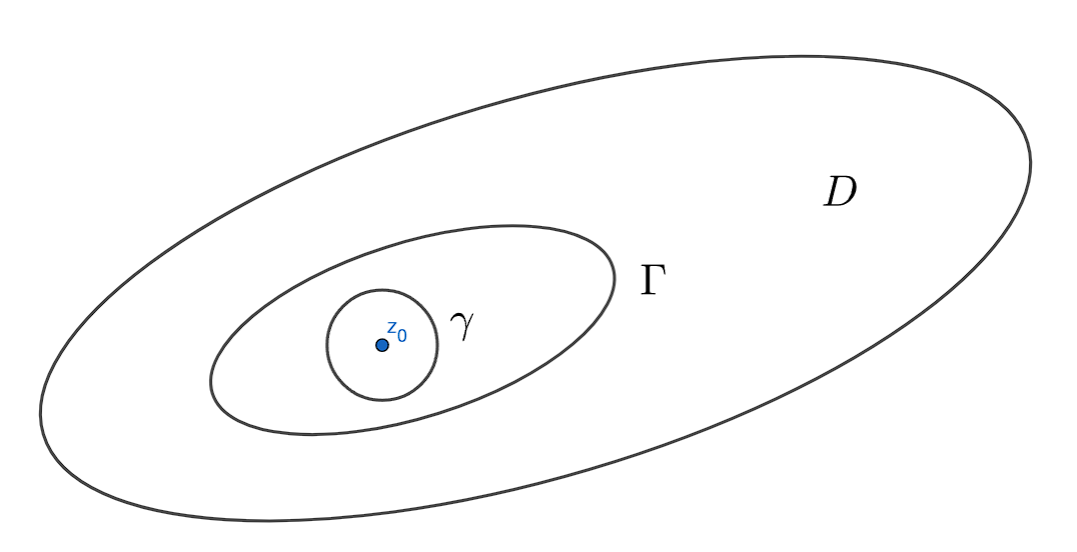
\includegraphics[width=7cm]{addchapters2/images/addchapters2_2025_04_04_5}
\end{wrapfigure}


\Nota Установим связь между щначениями $f(z)$ во внутренних точках области и на ее границе

$f(z)$ аналитична в обносвязной области $D$, $z_0 \in D$. Окружаем $z_0$ контуром $\Gamma \in D$ и меньшим контуром
$\gamma: |z - z_0| = \rho$

В кольце между $\gamma$ и $\Gamma$ рассмотрим функцию $\varphi(z) = \frac{f(z)}{z - z_0}$ (в кольце $\varphi(z)$ аналитична)

По \ThNs{2} для $\varphi(z)$ в многосвязной области $\int_{\Gamma \CounterClockwiseArrow} \varphi(\zeta) d\zeta = \int_{\gamma \CounterClockwiseArrow} \varphi(\zeta) d\zeta$ - не зависит от пути 

То есть выбор окружности в качестве $\gamma$ не важен:

$\int_{\gamma \CounterClockwiseArrow} \varphi(\zeta) d\zeta \overset{z - z_0 = \rho e^{i\varphi}}{=} \int_0^{2\pi} \frac{f(\zeta) \rho i e^{i\varphi} d\varphi}{\rho e^{i \varphi}} = i \int_0^{2\pi} f(\zeta) d\varphi = 
\underset{\text{стягиваем } \gamma \text{ в точку } z_0, \int \to 0}{\underbrace{i \int_0^{2\pi} (f(\zeta) - f(z_0)) d\zeta}} + i \int_0^{2\pi} f(z_0) d\zeta = i f(z_0) \cdot 2\pi$

Тогда $\int_\Gamma \frac{f(z)}{z - z_0} dz = \int_\gamma \varphi(\zeta) d\zeta = 2\pi i f(z_0)$

\Nota Доказали теорему: в области аналитичности $\forall z_0 \in D \ \int_{\Gamma_D} \frac{f(z)}{z - z_0} dz = 2 \pi i f(z_0)$

\Ex $\int_{|z| = 2 \CounterClockwiseArrow} \frac{f(z)}{(z - 1)(z + 1)} dz = \int_{|z - 1| = \rho_1 \CounterClockwiseArrow} \frac{\frac{f(z)}{z + 1}}{z - 1} dz + \int_{|z + 1| = \rho_2 \CounterClockwiseArrow} \frac{\frac{f(z)}{z - 1}}{z + 1} dz = 
2\pi i \left(\frac{f(1)}{2} + \frac{f(-1)}{-2}\right)$
